\documentclass{scrbook}
\usepackage{graphicx} % Required for inserting images
\usepackage{tabularx} % Required for fixed width tables
\usepackage{scrlayer-scrpage} % Required for the subtitles
\usepackage{url} % Required for the URLs
\usepackage{hyperref} % Required for the URLs
\usepackage{listings} % Required for the code snippets
\usepackage{mathtools} % Required for the system of equations
\usepackage{amsmath,amssymb} % Required for some math symbols
\usepackage{enumitem} % Required for lettered lists

% Put the caption of the snippets at the bottom
\lstset{
    captionpos=b
}


\title{Ethereum}
\subtitle{Ambient intelligence course (A.Y. 2025/2026)\\Topic taught by Prof. Arnaldo Tomasino}
\author{Gabriele Colapinto}
\date{\today}

\begin{document}

\maketitle
\thispagestyle{empty}

{\Large\textbf{License}} \\
{Notes from Ambient intelligence (A.Y. 2025/2026) by Gabriele Colapinto. 
Course taught by professors Michele Ruta, Floriano Scioscia, Arnaldo Tomasino, Davide Loconte — 
Licensed under CC BY-NC 4.0.\\
\url{https://creativecommons.org/licenses/by-nc/4.0/}}

\vspace*{\fill}
\rule{\textwidth}{0.2pt}
\small{© 2025 Gabriele Colapinto \\
Released under the \href{https://creativecommons.org/licenses/by-nc/4.0/}{Creative Commons Attribution–NonCommercial 4.0 International License}}

\clearpage

\tableofcontents

\chapter{Foundational Concepts of Ethereum}

Ethereum is a general-purpose, programmable blockchain that extends beyond the capabilities of earlier platforms designed primarily for financial transactions. Understanding its fundamental architecture—the platform itself, its native currency, and its execution environment—is essential before exploring its more complex mechanics and applications. This chapter provides a foundational overview of the Ethereum protocol, from its core concepts and motivations to the specific data structures that ensure its integrity.

\section{Defining Ethereum: The World Computer}

Ethereum is the world's largest programmable blockchain platform. It is an open-source project distributed under the GPLv3 license. Conceived as a "world computer," Ethereum is a general-purpose platform designed to support a wide range of applications that go far beyond simple financial transactions. Its native cryptocurrency, Ether (ETH), is not only a medium of exchange but also serves as the fuel for powering computation across the network.

\section{Core Applications: Smart Contracts and Decentralized Applications (Dapps)}

The core logic executed on the Ethereum blockchain is encapsulated in \textbf{smart contracts}. These immutable pieces of code are stored on the blockchain and run as programmed. Applications that use the blockchain as a back-end, leveraging smart contracts for their core functionality, are known as \textbf{Decentralized Applications (Dapps)}. \\

Because their logic is executed on-chain, Dapps possess three key properties:

\begin{itemize}
    \item \textbf{Trustworthiness:} Once deployed on Ethereum, a Dapp's smart contracts will run exactly as programmed, ensuring deterministic outcomes for given inputs.
    \item \textbf{Asset Control:} Dapps can be designed to manage and control digital tokenized assets with a high degree of precision.
    \item \textbf{Decentralization:} By their nature, Dapps are not controlled by any single entity or person.
\end{itemize}

The main application categories built on Ethereum include cryptocurrency wallets, financial applications, decentralized markets, and games where players can own and trade in-game assets.

\section{The Ethereum Virtual Machine (EVM)}

At the heart of Ethereum is the \textbf{Ethereum Virtual Machine (EVM)}, the execution environment where all smart contract code runs. Every node participating in the Ethereum network runs an instance of the EVM. \\

This design ensures that all nodes execute the exact same code, which is the mechanism for validating transactions and confirming state changes across the entire distributed system. Having established what Ethereum is at a high level, it is useful to understand why it was created and how it evolved from its predecessors.

\chapter{The Genesis and Motivation of Ethereum}

Ethereum was not developed in a vacuum; it was created as a direct response to the perceived limitations of earlier blockchain platforms, most notably Bitcoin. Its design was motivated by a desire to build a more flexible and general-purpose blockchain.

\section{A Brief History}

Ethereum's development can be traced through several key milestones:

\begin{itemize}
    \item \textbf{2013:} Vitalik Buterin first proposed the concept in a white paper.
    \item \textbf{December 2013:} Buterin, along with four other founders, established the Ethereum.org non-profit organization.
    \item \textbf{2014:} The founders established Ethereum Switzerland GmbH and began software development.
    \item \textbf{July 30, 2015:} The first stable release of the Ethereum software was launched.
    \item \textbf{Post-2015:} The protocol has undergone several changes through soft and hard forks to add new features, combat attacks, and improve overall security.
\end{itemize}

\section{Why Ethereum? Analyzing the Limitations of Bitcoin}

The development of Ethereum was driven by the goal of overcoming four primary limitations observed in the Bitcoin protocol.

\begin{enumerate}
    \item \textbf{Lack of Turing-Completeness} A computational system is considered Turing-complete if it can perform a wide range of general-purpose operations, such as loops and conditionals, allowing it to implement complex algorithms. Bitcoin’s scripting language is not Turing-complete; for example, it completely lacks constructs for loops. This severely limits its functionality. Ethereum was designed with more general-purpose scripting languages, like Solidity, which are Turing-complete and enable the development of far more sophisticated applications.
    
    \item \textbf{Value-Blindness} Bitcoin’s Unspent Transaction Output (UTXO) model is "all-or-nothing." A UTXO script cannot provide fine-grained control over the amount of currency that can be withdrawn from an output; the entire UTXO must be consumed in a transaction. In contrast, Ethereum's account-based model allows for more direct and precise value transfers, where any desired amount can be sent from an account's balance, provided the funds are sufficient.
    
    \item \textbf{Lack of State} The all-or-nothing nature of the UTXO model means that multi-stage contracts or scripts cannot maintain an internal state between transactions. For example, a contract that requires a timeout or depends on multiple conditions being met over time is not feasible. Ethereum solves this with stateful smart contracts, where data can be stored and updated within the contract itself, enabling advanced protocols and applications.
    
    \item \textbf{Blockchain-Blindness} In Bitcoin, UTXO-based transactions cannot access blockchain data such as the nonce or the hash of a previous block. Ethereum allows smart contracts to access this on-chain data, which can be used as a source of randomness for applications like games and gambling.
\end{enumerate}

These motivations led to a fundamental architectural shift away from the UTXO model and toward an account-based system.

\chapter{The Ethereum Account Model}

Unlike Bitcoin's UTXO ledger, Ethereum's state is defined by the properties of all existing accounts. Every change to the network is a transition from one state to another, driven by interactions between these accounts. \\

This account-based architecture was a direct solution to the limitations of value-blindness and lack of state inherent in Bitcoin's UTXO model, enabling the stateful, multi-stage contracts that were previously impossible.


\section{The Two Types of Accounts}

Ethereum features two distinct types of accounts, each with a unique purpose and control mechanism.

\begin{table}[h]
    \centering
    \begin{tabular}{|p{0.45\textwidth}|p{0.45\textwidth}|}
    \hline
    \textbf{Externally Owned Account (EOA) / User Account} & \textbf{Contract Account / Smart Contract} \\
    \hline
    Controlled by a private key. & Controlled by its contract code. \\
    \hline
    Represents a regular user account. & Represents a smart contract. \\
    \hline
    Activated by creating and signing a transaction. & Activated when it receives a message or transaction. \\
    \hline
    Can create new contracts. & Can create other contracts via its code. \\
    \hline
    \end{tabular}
    \caption{Comparison of Ethereum Account Types}
\end{table}

\section{The Structure of an Account}

\begin{figure}
    \centering
    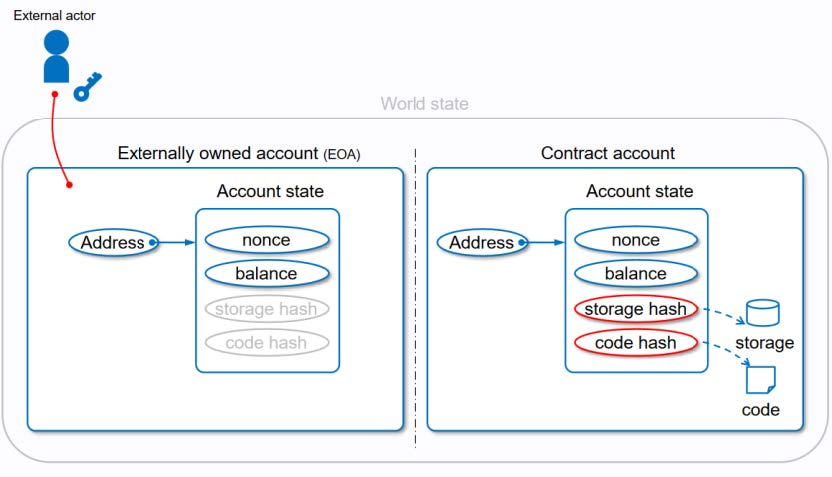
\includegraphics[width=\linewidth]{Images/Ethereum_accounts.jpg}
    \caption{Ethereum accounts}
    \label{fig:ethereum_accounts}
\end{figure}

Every account in Ethereum, whether an EOA or a contract, is defined by four fields (see figure \ref{fig:ethereum_accounts}):

\begin{enumerate}
    \item \textbf{Nonce:} This field acts as a counter of transactions sent from the account. It is distinct from the nonce used in Proof-of-Work. Its purpose is to ensure that each transaction can only be processed once and that transactions are processed in the correct sequential order.
    
    \item \textbf{Balance:} This field stores the account's current balance in Ether or its sub-denominations, such as Wei ($10^{-18}$ ETH) or Gwei ($10^{-9}$ ETH).
    
    \item \textbf{Contract Code:} For a contract account, this field contains the compiled smart contract code. For an EOA, this field is empty.
    
    \item \textbf{Storage:} This is the account's persistent storage, organized as a key-value store. It is empty by default and is only used by contract accounts to maintain state.
\end{enumerate}

Changes to these account fields are driven by transactions initiated by external actors and messages generated by contracts.

\chapter{The Mechanics of Execution: Transactions, Messages, and Gas}

Transactions are the fundamental drivers of all state changes in the Ethereum network. This section deconstructs the components of a transaction, explains how contracts communicate with each other, and details the critical resource management mechanism known as Gas.

\section{Transactions: The Catalyst for State Change}

\begin{figure}
    \centering
    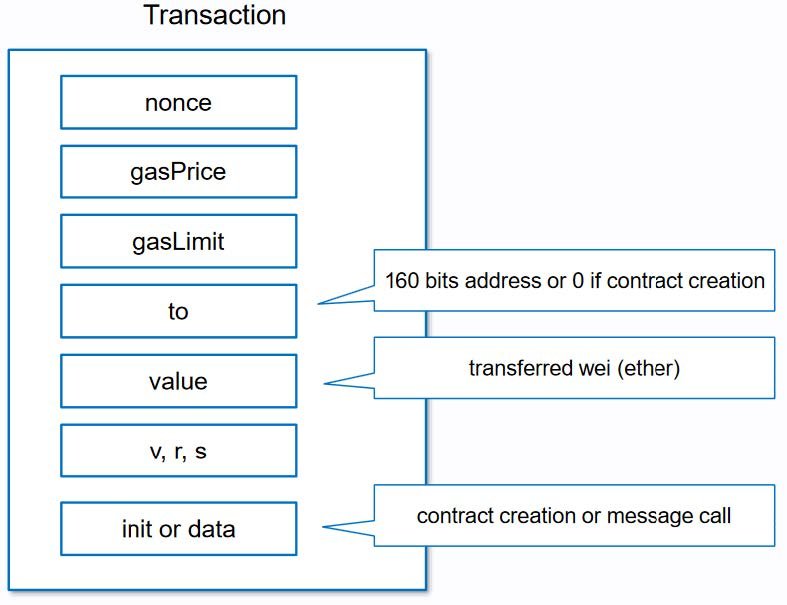
\includegraphics[width=0.5\linewidth]{Images/Transactions.jpg}
    \caption{Ethereum transaction data}
    \label{fig:ethereum_transaction_data}
\end{figure}

A transaction in Ethereum is a signed data package that stores a message sent from an account. It contains several key fields (see figure \ref{fig:ethereum_transaction_data}):

\begin{itemize}
    \item \textbf{Signature:} Identifies the sender of the transaction. In Ethereum, the signature is represented by the three values \texttt{v}, \texttt{r}, and \texttt{s}, which are the components of an ECDSA (Elliptic Curve Digital Signature Algorithm) signature:
    \begin{itemize}
        \item \textbf{\texttt{r}:} The first component of the ECDSA signature.
        \item \textbf{\texttt{s}:} The second component of the ECDSA signature, computed from the transaction hash, the sender's private key, and an ephemeral cryptographic nonce.
        \item \textbf{\texttt{v}:} The recovery identifier, used to recover the sender's public key from the signature. In legacy Ethereum transactions it was typically \texttt{27} or \texttt{28}; with EIP-155 it also encodes the chain ID to protect against replay attacks across different chains.
    \end{itemize}
    \item \textbf{to:} The 20-byte destination address.
    \item \textbf{value:} The amount of Ether to transfer from the sender to the recipient.
    \item \textbf{data:} An optional field that can contain data for contract interaction.
    \item \textbf{nonce:} The anti-replay value, which corresponds to the sending account's nonce.
    \item \textbf{gasLimit (or startgas):} The maximum number of computational steps the transaction and all its sub-executions are allowed to take.
    \item \textbf{gasPrice:} The fee, in Ether, that the sender agrees to pay for each computational step.
\end{itemize}

There are three primary types of transactions:

\begin{enumerate}
    \item \textbf{Regular transactions:} A simple transfer of Ether from one account to another.
    \item \textbf{Contract execution:} A transaction sent to a contract account's address, which triggers the execution of the contract's code.
    \item \textbf{Contract deployment:} A transaction where the \texttt{to} field is empty (or a null address) and the \texttt{data} field contains the compiled bytecode of a smart contract. Upon execution, this transaction creates a new contract account, populates it with the code, and assigns it a unique address.
\end{enumerate}

\subsection{Clarifying the transaction signature}

In Ethereum, a transaction is authenticated through an ECDSA signature generated by the sender. The signature consists of three values: \texttt{r}, \texttt{s}, and \texttt{v}.

Consider the following example signature associated with a transaction:

\begin{itemize}
    \item \texttt{r = 0x1c3a\ldots 8f21}
    \item \texttt{s = 0x5b72\ldots c914}
    \item \texttt{v = 28}
\end{itemize}

The signature is generated as follows:

\begin{enumerate}
    \item The sender prepares the transaction fields such as the recipient address, value, data, nonce, and gas parameters.
    \item The sender computes the hash of the transaction data.
    \item Using their private key, the sender signs this hash with the ECDSA algorithm over the \texttt{secp256k1} curve.
    \item The signing algorithm produces the values \texttt{r} and \texttt{s}.
    \item An additional value, \texttt{v}, is included as a recovery identifier.
\end{enumerate}

When the transaction is received by a node, the signature is interpreted as follows:

\begin{enumerate}
    \item The node recomputes the hash of the received transaction.
    \item The node uses \texttt{v}, \texttt{r}, and \texttt{s} to recover the sender's public key.
    \item The Ethereum address is derived from the recovered public key.
    \item The node verifies that the signature is valid and that the recovered address corresponds to the claimed sender.
\end{enumerate}

Therefore, the tuple \texttt{(v, r, s)} allows Ethereum nodes to verify both the authenticity and the integrity of the transaction without requiring the sender to explicitly transmit their public key.

\section{Messages: Contract-to-Contract Communication}

Messages are similar to transactions (they contain an implicit sender, \texttt{to}, \texttt{value}, optionally \texttt{data} and \texttt{startgas}) but are produced by contracts, not by external actors. When one smart contract needs to interact with another, it does so by sending a message (for example, using the \texttt{CALL} opcode in the EVM). Crucially, messages are \textbf{virtual objects} that exist only within the Ethereum execution environment. They are never serialized or stored on the blockchain itself.

\section{Gas: The Fuel for the Ethereum Network}

\begin{figure}
    \centering
    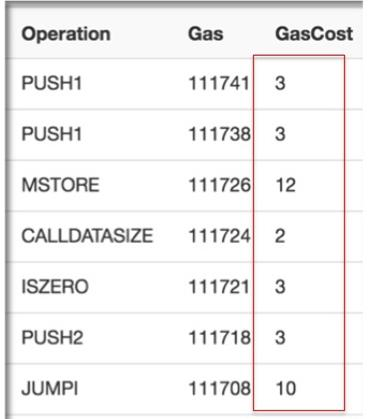
\includegraphics[width=0.5\linewidth]{Images/Gas.jpg}
    \caption{Example of EVM execution trace associating to each operation the current gas of the execution and the gas consumed by each operation}
    \label{fig:EVM_execution_trace}
\end{figure}

Gas is the unit that measures the amount of computational effort required to execute operations on the Ethereum network. It serves two primary purposes:

\begin{enumerate}
    \item \textbf{Resource Payment:} To ensure that all consumed resources—including computation, bandwidth, and storage—are paid for by the transaction sender.
    \item \textbf{Preventing Wastage:} To prevent infinite loops or other forms of computational waste by imposing a hard limit (\texttt{gasLimit}) on the total computation a transaction can perform.
\end{enumerate}

The \texttt{transaction fee} is calculated by multiplying the gas price by the amount of gas consumed (\texttt{gasPrice * consumedGas}). If a transaction's execution requires more computation than the specified \texttt{gasLimit}, it triggers an "Out of gas exception". In this event, the transaction is reverted, but the sender is still required to pay for the gas that was consumed up to the limit.\\

These mechanics of transactions, messages, and gas are formalized in the Ethereum state transition function, which governs how the blockchain's state evolves.

\subsection{Clarification of figure \ref{fig:EVM_execution_trace}}

The table represents an execution trace of the Ethereum Virtual Machine (EVM). Each row corresponds to an opcode executed by the EVM, such as \texttt{PUSH1}, \texttt{MSTORE}, or \texttt{JUMPI}. The \texttt{GasCost} column indicates the amount of gas consumed by that specific instruction, while the \texttt{Gas} column indicates the amount of gas remaining at that point during execution.\\

Therefore, the table should not be interpreted as showing the sender's gas directly, but rather the gas budget still available to the EVM while executing the transaction or contract call. This gas budget initially comes from the transaction's gas limit and is reduced step by step as each opcode is executed.\\

For example, if one row shows \texttt{PUSH1} with \texttt{GasCost = 3}, and the following row reports that the remaining gas has decreased by 3, this means that the execution of that opcode consumed exactly 3 units of gas. In this sense, the trace provides a detailed view of how gas is spent throughout the execution of the bytecode.\\

It is also important to note that the gas cost of an opcode is not always fixed. While some instructions have a constant cost, others may have a variable cost depending on the execution context, for example due to storage access or memory expansion. Memory expansion in the EVM refers to the increase of the temporary linear memory used during contract execution. When an instruction accesses a memory region beyond the highest previously used offset, the EVM expands the memory and charges an additional gas cost. Therefore, the cost of some opcodes depends not only on the instruction itself, but also on whether executing it requires allocating more memory.

\chapter{The Ethereum State Transition Function}

\begin{figure}
    \centering
    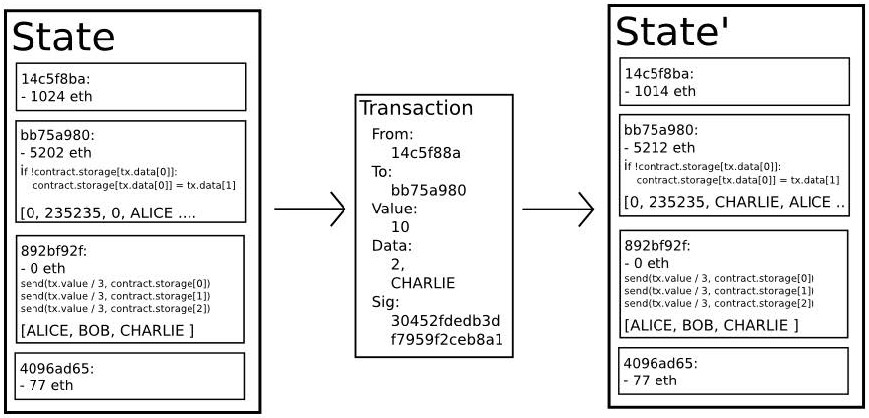
\includegraphics[width=\linewidth]{Images/State_transitions.jpg}
    \caption{Ethereum state transitions}
    \label{fig:state_transitions}
\end{figure}

At its core, every blockchain is a state transition system. The state of Ethereum is formally defined as the complete set of all existing accounts and their properties (balance, nonce, code, and storage). State changes are formalized by the Ethereum state transition function, represented as:

\begin{center}
$APPLY(S, TX) \rightarrow S'$
\end{center}

This equation signifies that a new state \texttt{S'} is produced by applying a transaction \texttt{TX} to the current state \texttt{S} (see figure \ref{fig:state_transitions}).

\section{The State Transition Process}

The state transition function follows a precise, step-by-step process for each transaction:

\begin{enumerate}
    \item \textbf{Validation:} The function first checks whether the transaction is well-formed, for example whether the signature is valid and whether the transaction format is correct. Some preliminary checks may also be performed locally by a wallet or client before the transaction is broadcast. However, checks that depend on the current blockchain state, such as the sender's balance or nonce, can only be definitively verified by network nodes against the current state. Local preliminary checks do not consume gas on-chain.

    \item \textbf{Fee Pre-payment:} The maximum transaction fee is determined from the gas limit and the fee parameters of the transaction. In legacy transactions this corresponds to \texttt{startgas * gasprice}. This maximum amount is reserved from the sender's balance, and the sender's account nonce is incremented. If the sender's balance is insufficient to cover the maximum possible cost and the transferred value, the transaction is rejected.

    \item \textbf{Gas Initialization:} A \texttt{gas} counter for the transaction is initialized to the \texttt{startgas} (or \texttt{gasLimit}) value. A preliminary intrinsic gas cost, based on the transaction itself (for example its base cost and the size of its input data), is immediately deducted.

    \item \textbf{Execution:} The transaction is executed by the EVM. If the transaction transfers Ether to an externally owned account, the value is transferred directly. If the recipient is a contract account, the contract code is executed until it either completes successfully, triggers a revert, or runs out of gas. During execution, each opcode consumes gas according to its computational cost.

    \item \textbf{Finalization (Success):} If execution completes successfully, the unused gas is refunded to the sender. The sender ultimately pays only for the gas that was actually consumed. The corresponding transaction fee is then distributed according to the protocol rules.

    \item \textbf{Finalization (Failure):} If execution fails, for example because of an exception, a revert, or an out-of-gas condition, the state changes produced by execution are reverted. However, the transaction itself remains recorded on the blockchain if it has been included in a block, the sender's nonce remains incremented, and the gas consumed during execution is still charged. Thus, a failed transaction may have no intended effect on the application state, while still costing Ether in transaction fees.
\end{enumerate}

It is important to distinguish between \emph{gas} and \emph{Ether}. Gas is not a currency stored in the network, but a unit used to measure computational effort in the EVM. Transaction fees are paid in Ether according to the amount of gas consumed. Therefore, gas itself is not transferred between accounts and there is no fixed ``quantity of gas'' in the system.

More precisely, the transaction fee is computed from the gas used and the fee parameters of the transaction. In modern Ethereum, part of the fee may be burned by the protocol, while another part may be assigned to the block proposer as compensation. Consequently, the total amount of Ether in circulation is not constant merely because transaction fees are paid within the network.

\chapter{Data Structures: Blocks and Merkle-Patricia Trees}

The integrity and efficiency of the Ethereum blockchain depend on specific data structures designed for cryptographic verification. This section examines the composition of an Ethereum block and the crucial role of the Merkle-Patricia tree in securing state and transaction data.

\section{The Structure of an Ethereum Block}

\begin{figure}
    \centering
    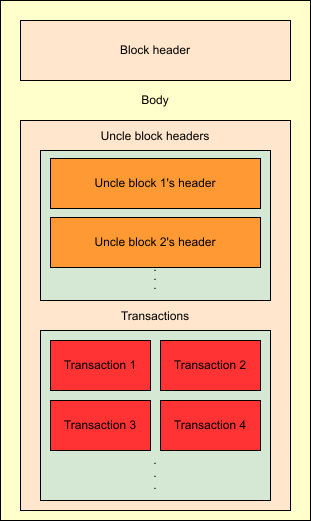
\includegraphics[width=0.5\linewidth]{Images/Ethereum block.png}
    \caption{Ethereum block}
    \label{fig:ethereum_block}
\end{figure}

An Ethereum block consists of a header and a list of transactions (see figure \ref{fig:ethereum_block}). The header contains several key fields:

\begin{itemize}
    \item \textbf{Parent's Block Hash:} A hash that links the current block to the previous block, forming the chain.
    
    \item \textbf{Uncle Block's Hash:} The hash of an "uncle block." An uncle block is a block that was mined at the same time as the parent but was not included in the chain. Including its hash serves protocol-related purposes such has not wasting computational work to make the system fairer. The miner of the uncle block is partially rewarded for their computational effort and also the miner of the main block is rewarded for including the hash of the uncle block in the header.
    
    \item \textbf{State Root Hash:} The root hash of the Merkle-Patricia tree that represents the entire state of the system \textit{after} all transactions in the block have been executed.
    
    \item \textbf{Transaction Root Hash:} The root hash of the Merkle-Patricia tree containing all transactions included in the block.
\end{itemize}

The list of transactions itself is also included in the block, encoded using Recursive Length Prefix Encoding (RLP).

\section{The Merkle-Patricia Tree}

The \textbf{Merkle-Patricia tree} (also known as a radix tree or trie) is the core data structure used in Ethereum to store and verify key-value mappings for both the state and transactions. Its key features are:

\begin{itemize}
    \item It is a type of prefix tree where the path to a value is determined by its key (e.g., an account address determines the path to that account's data).
    \item Each node in the tree is referenced by its cryptographic hash.
    \item The single \textbf{root node's hash} serves as a unique cryptographic proof, or fingerprint, of the entire dataset contained within the tree.
\end{itemize}


The significance of this structure is profound. Any change to a single piece of data, such as an account's balance, will propagate up the tree and result in a different root hash. This makes it extremely efficient for nodes to verify that the state has changed between blocks by simply comparing a single 32-byte root hash.

\chapter{Defining Token Systems on Ethereum}

Formally, a token system is a database, backed by the blockchain, defined by a single fundamental operation: subtracting a number of units from account A and adding the same number to account B. This operation is governed by two essential conditions:

\begin{enumerate}
    \item The sending account (A) must possess at least the number of units being transferred.
    \item The transaction must be explicitly approved by the sender (A).
\end{enumerate}

While this sounds simple, it enables a wide array of applications. The logic for these systems is encoded within smart contracts, allowing for the creation of diverse digital assets and functionalities.

\begin{itemize}
    \item \textbf{Sub-currencies:} Tokens can represent other assets, such as fiat currency (e.g., Euros), commodities (e.g., gold), or financial instruments like company stocks.
    \item \textbf{Smart Property:} Individual, unique tokens can represent ownership of real-world property, creating a secure and verifiable digital title.
    \item \textbf{Unforgeable Coupons:} Secure, verifiable digital coupons that can be issued and redeemed on the blockchain.
    \item \textbf{Incentivization Systems:} Points systems can be created for gamification, rewards programs, or other incentivization models.
\end{itemize}

\section{Token Standards: A Framework for Interoperability}

To ensure that the vast number of tokens created on Ethereum can interact seamlessly, the community has developed token standards. These standards are strategic frameworks that allow developers to build interoperable applications—such as wallets and decentralized exchanges—that can regulate the exchange of different tokens in a uniform and predictable way. The two most prominent standards are ERC-20 for fungible tokens and ERC-721 for non-fungible tokens.

\subsection{ERC-20: The Standard for Fungible Tokens}

ERC-20 is the most widespread token standard on Ethereum, defining the interface for \textbf{fungible tokens}. Fungibility means that each unit of a token is identical and interchangeable with any other unit, much like how one banknote of a certain value is interchangeable with any other banknote of the same value. \\

The name "ERC-20" originates from its status as the 20th "Ethereum Request for Comments," a community process for proposing protocol improvements. This system has since evolved into the "Ethereum Improvement Proposal" (EIP) framework, but the original name for this popular standard has remained.\\

The ERC-20 interface specifies a set of core functions that a compliant smart contract must implement. These functions are listed in table \ref{tbl:erc20_interface_functions}.

\begin{table}[h]
    \centering
    \begin{tabularx}{\linewidth}{|p{20em}|X|}
    \hline
    \textbf{Function} & \textbf{Description} \\
    \hline
    \texttt{name()} & Returns the name of the token. \\
    \hline
    \texttt{symbol()} & Returns the symbol of the token. \\
    \hline
    \texttt{decimals()} & Returns the number of decimals the token uses. \\
    \hline
    \texttt{totalSupply()} & Returns the total supply of the token. \\
    \hline
    \texttt{balanceOf(address \_owner)} & Returns the account balance of a specified owner. \\
    \hline
    \texttt{transfer(address \_to, uint256 \_value)} & Transfers a specified amount of tokens to a destination address. \\
    \hline
    \end{tabularx}
    \caption{ERC-20 Interface Functions}
    \label{tbl:erc20_interface_functions}
\end{table}

\subsection{ERC-721: The Standard for Non-Fungible Tokens (NFTs)}

ERC-721 is the official interface for \textbf{non-fungible tokens (NFTs)}. Unlike fungible tokens, each NFT is unique and not interchangeable. This standard gained prominence with the CryptoKitties game and is now widely used to represent ownership of unique digital or physical assets, such as digital art, collectibles, or in-game items.

The ERC-721 standard includes functions for tracking ownership and managing transfers of these unique assets. These functions are listed in table \ref{tbl:erc721_interface_functions}.

\begin{table}[h]
    \centering
    \begin{tabularx}{\linewidth}{|p{20em}|X|}
    \hline
    \textbf{Function} & \textbf{Description} \\
    \hline
    \texttt{balanceOf(address \_owner)} & Returns the account balance of a specified owner.\\
    \hline
    \texttt{ownerOf(uint256 \_tokenId)} & Returns the address of the owner of a specific NFT.\\
    \hline
    \texttt{transferFrom(address \_from, address \_to, uint256 \_tokenId)} & Transfers ownership, but the caller is responsible for confirming the recipient's reception capability. If the recipient is not capable of receiving the NFT, it may be permanently lost.\\
    \hline
    \texttt{safeTransferFrom(address \_from, address \_to, uint256 \_tokenId [, bytes data])} & Transfers ownership of an NFT and performs checks to ensure the recipient can receive it.\\
    \hline
    \texttt{approve(address \_approved, uint256 \_tokenId)} & Grants another address permission to manage a specific NFT.\\
    \hline
    \texttt{getApproved(uint256 \_tokenId)} & Retrieves the approved address for a specific NFT.\\
    \hline
    \texttt{setApprovalForAll(address \_operator, bool \_approved)} & Enables or disables a third-party "operator" to manage all of the caller's assets.\\
    \hline
    \texttt{isApprovalForAll(address \_owner, address \_operator)} & Queries if an address is an authorized operator for another address.\\
    \hline
    \end{tabularx}
    \caption{ERC-721 Interface Functions}
    \label{tbl:erc721_interface_functions}
\end{table}

\section{The Evolution of the Ethereum Protocol}

Ethereum is not a static protocol. It undergoes significant updates to address critical challenges, most notably scalability and energy consumption, ensuring its long-term viability and performance.

\subsection{The Merge: Transition to Proof of Stake}

"The Merge" was a major protocol update where Ethereum transitioned its consensus mechanism from Proof of Work (PoW) to Proof of Stake (PoS). This monumental shift was driven by two primary goals: increasing transaction throughput and drastically reducing the computational costs and energy consumption associated with network security.

This update was successfully completed on \textbf{September 15, 2022}. All blocks from number 15537393 onwards have been created using the PoS consensus model.

\subsection{Sharding: A Proposed Solution for Scalability}

Sharding is a proposed solution designed to address Ethereum's scalability issues. The core mechanism involves dividing the entire network into smaller, more manageable subnetworks called "shards." In this model, each node is only required to store and manage a fraction of the entire blockchain (its assigned shard) rather than the complete dataset. \\

This approach presents a trade-off between scalability and complexity, with several key benefits and drawbacks.


\begin{itemize}
    \item \textbf{Benefit:} Allows the network to scale up as it grows by significantly reducing the storage and processing requirements for individual nodes.
    \item \textbf{Drawback:} Requires additional coordination algorithms to manage communication and state consistency across shards, which can introduce latency.
    \item \textbf{Drawback:} The increased complexity and potential latency may negatively affect the usability and performance of certain applications.
    \item \textbf{Drawback:} The sharded architecture may not be compatible with all existing applications, potentially requiring them to be redesigned.
\end{itemize}

\end{document}
